\documentclass{standalone}
\usepackage{graphicx}	
\usepackage{amssymb, amsmath, amsthm}
\usepackage{color}

\usepackage{tikz}
\usetikzlibrary{intersections, backgrounds, math}

\definecolor{light}{RGB}{220, 188, 188}
\definecolor{mid}{RGB}{185, 124, 124}
\definecolor{dark}{RGB}{143, 39, 39}
\definecolor{highlight}{RGB}{180, 31, 180}
\definecolor{lightteal}{RGB}{186, 219, 219}
\definecolor{midteal}{RGB}{124, 186, 186}
\definecolor{darkteal}{RGB}{38, 142, 142}
\definecolor{darkerteal}{RGB}{0, 124, 124}
\definecolor{gray10}{gray}{0.1}
\definecolor{gray20}{gray}{0.2}
\definecolor{gray30}{gray}{0.3}
\definecolor{gray40}{gray}{0.4}
\definecolor{gray60}{gray}{0.6}
\definecolor{gray70}{gray}{0.7}
\definecolor{gray80}{gray}{0.8}
\definecolor{gray90}{gray}{0.9}
\definecolor{gray95}{gray}{0.95}

\newcommand{\fiber}[2]{
  \pgfmathsetmacro{\x}{#1}
  \draw [color=#2, line width=1]
      (\x, -2) .. controls (\x - 0.75, -1) and (\x + 0.5, -0.25) 
   .. (\x + 0.5, 0.25) .. controls (\x + 0.5, 0.75) and (\x - 0.5, 1.25) .. (\x + 0.25, 2)
}

\begin{document}

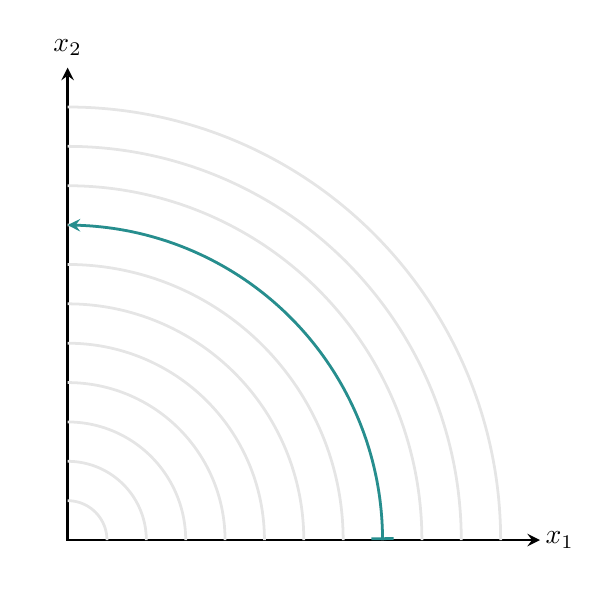
\begin{tikzpicture}[scale=1]
   
  \draw[white] (-3.5, -3.5) rectangle (3.5, 3.5);
   
  \draw[->, >=stealth, line width=1] (-3.015, -3) -- (3, -3);
  \node at (3.25, -3) { $x_{1}$ };  
  
  \draw[->, >=stealth, line width=1] (-3, -3) -- (-3, 3);
  \node at (-3, 3.25) { $x_{2}$ };  
  
  \begin{scope}
    \clip[rounded corners=5] (-3, -3) rectangle (3, 3);
   
    \foreach \r in {0.5, 1.0, ..., 5.5} { 
      \draw[domain=0:90, -, >=stealth, smooth, samples=50, variable=\th, gray90, line width=1] 
        plot ({\r * cos(\th) - 3}, {\r * sin(\th) - 3}); 
    }
  \end{scope}
  
  \draw[domain=0:90, |->, >=stealth, smooth, samples=50, variable=\x, darkteal, line width=1] 
        plot ({4 * cos(\x) - 3}, {4 * sin(\x) - 3});
  
   
\end{tikzpicture}

\end{document}  